% This file was created with tikzplotlib v0.10.1.
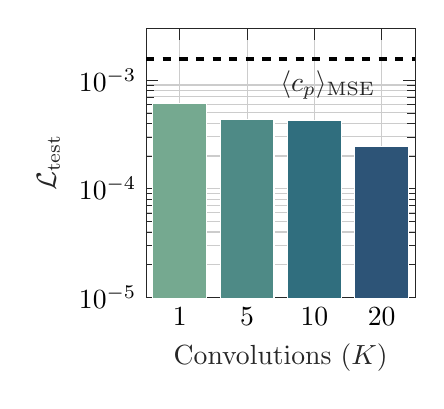
\begin{tikzpicture}

\definecolor{cadetblue117169144}{RGB}{117,169,144}
\definecolor{darkslategray38}{RGB}{38,38,38}
\definecolor{darkslategray4584119}{RGB}{45,84,119}
\definecolor{darkslategray66}{RGB}{66,66,66}
\definecolor{lightgray204}{RGB}{204,204,204}
\definecolor{seagreen48110126}{RGB}{48,110,126}
\definecolor{slategray78138134}{RGB}{78,138,134}

\begin{axis}[
width=5cm,
height=5cm,
axis line style={darkslategray38},
log basis y={10},
tick align=inside,
unbounded coords=jump,
x grid style={lightgray204},
xlabel=\textcolor{darkslategray38}{Convolutions (\(\displaystyle K\))},
xmajorticks=true,
xmin=-0.5, xmax=3.5,
xminorgrids,
xmajorgrids,
xtick style={color=darkslategray38},
xtick={0,1,2,3},
xticklabels={1,5,10,20},
y grid style={lightgray204},
ylabel=\textcolor{darkslategray38}{\(\displaystyle \mathcal{L}_{\mathrm{test}}\)},
ymajorticks=true,
% ymin=0.000224240305144263, ymax=0.00171444631116674,
ymin=1e-5, ymax=0.003,
yminorgrids,
ymode=log,
ytick style={color=darkslategray38},
% ytick={1e-05,0.0001,0.001,0.01,0.1},
% yticklabels={
%   \(\displaystyle {10^{-5}}\),
%   \(\displaystyle {10^{-4}}\),
%   \(\displaystyle {10^{-3}}\),
%   \(\displaystyle {10^{-2}}\),
%   \(\displaystyle {10^{-1}}\)
% }
]

\def\epsVal{1e-8}

\draw[draw=white,fill=cadetblue117169144] (axis cs:-0.4,\epsVal) rectangle (axis cs:0.4,0.000608911854214966);
\draw[draw=white,fill=slategray78138134] (axis cs:0.6,\epsVal) rectangle (axis cs:1.4,0.000430749409133568);
\draw[draw=white,fill=seagreen48110126] (axis cs:1.6,\epsVal) rectangle (axis cs:2.4,0.000420872267568484);
\draw[draw=white,fill=darkslategray4584119] (axis cs:2.6,\epsVal) rectangle (axis cs:3.4,0.000245962379267439);
\addplot [line width = 1.5pt, dashed, black]
table {%
-0.5 0.00156303563624041
3.5 0.00156303563624041
};
\addplot [line width=1.08pt, darkslategray66]
table {%
0 nan
0 nan
};
\addplot [line width=1.08pt, darkslategray66]
table {%
1 nan
1 nan
};
\addplot [line width=1.08pt, darkslategray66]
table {%
2 nan
2 nan
};
\addplot [line width=1.08pt, darkslategray66]
table {%
3 nan
3 nan
};
\draw (axis cs:1.35,0.0009) node[
  scale=1,
  anchor=west,
  text=darkslategray38,
  rotate=0.0
]{$ \langle c_p \rangle _ {\mathrm{MSE}}$};
\end{axis}

\end{tikzpicture}